\documentclass[fleqn,10pt]{wlscirep}
\usepackage[utf8]{inputenc}
\usepackage[T1]{fontenc}
\usepackage{graphicx}
\usepackage{url}
\usepackage{float}

\title{Scaffolding Student-AI Dialogue: A Framework for Safe Educational Interactions}

\author[1,+,*]{Olga Muss}
\author[2,+]{Luca M. Leisten}
\author[3]{Charles Edouard Bardyn}
\affil[1]{Université de Neuchâtel, ETH Zurich}
\affil[2]{ETH Zurich}
\affil[3]{AI Swiss}

\affil[*]{olga.muss@unine.ch}

\affil[+]{these authors contributed equally to this work}

\keywords{AI safety, education technology, language models, reliability engineering, verification, quality education (SDG 4)}

\begin{abstract}
Adolescents are the fastest and largest age group adopting the use of Large Language Models (LLMs), models that haven’t been specifically developed for them with their educational, emotional and developmental needs in mind. Safe, adapted and appropriate LLMs are essential for AI literacy, as well as for the safe and beneficial use in educational settings and beyond. We present SCAFFOLD, a layered reliability framework that surrounds generation with external verification, targeted repair, and safe fallback that could work with any model and enable data privacy. Grounded in pedagogical and developmental analysis, it starts by designing the interaction for a context and a goal, then defines guidance and checks to be implemented. It distinguishes deterministic checks from statistical checks. We test the approach in classroom deployment with 13–15-year-old students using a LLM-powered social robot in a multi-user interaction of co-creation of a mnemonic on a topic covered previously. Each group interacted with a prompt-only baseline and then with the full framework. The students were much more active, engaged and on topic with the framework and co-creation effort predicted post-test knowledge scores, showing potential of the framework to support engagement, social interactions and learning.
\end{abstract}

\begin{document}

\flushbottom
\maketitle
\thispagestyle{empty}

\section*{1 Introduction}

Generative Artificial Intelligence (AI) in the form of Large Language Models (LLMs) used in AI chatbots has been transformative in the last few years with a rapid adoption of AI chatbots by the general public and particularly young users. In Switzerland, 84\% of 14–19-year-olds report regular use of generative AI (survey of 1,100 Swiss residents, 2025) the highest usage of any other age group, while only 60\% of 30–49-year-olds and less than 40\% of 50–69-year-olds reporting regular AI use \cite{WIP-CH2025}. In the United Kingdom, 53\% of 9–11-year-olds and 67\% of 15–17-year-olds report regular use of AI chatbots \cite{InternetMatters2025}. This is no surprise, since AI chatbots are now embedded  in apps that children and adolescents use, such as snapchat, whatsapp, tiktok, or instagram.

The risks of using LLMs are numerous, from data privacy concerns and unsafe responses to attachment, cognitive atrophy and over-trust (Neugnot-Cerioli \& Muss Laurenty, 2024, Kurian, 2025, UNESCO, 2021, VIOLA DE AZEVEDO CUNHA, 2017, Yu, 2025, Chandra et al., 2025 pre-print). While society as a whole needs to address these issues, the educational sector faces specific challenges, as it simultaneously has to educate students about AI technologies and protect them from harm (\textit{United Nations Convention on the Rights of the Child}, 1989) – a duty even more critical when considering that children's knowledge is limited and their brains are still developing (Gogtay et al., 2004). To realize the potential benefits of generative AI tools for education and young people's lives (UNESCO, 2021), we need to ensure that these tools are safe and developmentally adapted to their users.

To achieve this goal and thereby protect children from harmful AI interactions both conceptual and technical work is needed: conceptual work defines what it means that student \- AI interactions are safe and developmentally appropriate, while technical work deals with steering of LLMs behaviors. Here we present a methodology \- \textbf{SCAFFOLD (Steered Contextual AI Framework for Orchestrating Learning Dialogue)} \- whose goal is to enable alignment of pedagogical goals with technical feasibility in the educational context of student \- AI interactions. In this paper we first present the general concept of the framework highlighting its potential, then we present a minimal version of the frame and the results of a pilot study in a STEM context  with 12-15 year olds. The contributions of this paper are:

\begin{itemize}
\item A novel \textbf{SCAFFOLD (Steered Contextual AI Framework for Orchestrating Learning Dialogue)} methodology that allows to steer LLM behavior to comply with a designed AI- student interaction and to increase LLM reliability at a level necessary to allow the responsible deployment in schools and beyond.
\item A \textbf{developed modular system of frames} for co-creating a mnemonic in multi-user interaction with an AI with balanced turns management, contribution tracking, phases and time management, that is available open source.
\item \textbf{Empirical testing results} in a classroom deployment with 12–15-year-old students showing feasibility and potential to support learning.
\end{itemize}

\section*{2 A framework for safe LLM interactions}

AI \- student interaction is a dynamic process involving feedback loops that reinforce or discourage certain behaviors in a multi-turn dialogue. It is therefore necessary to design these interactions with the desired flow in mind, building on the science of learning and pedagogy. It is also necessary to steer LLM's behavior at each turn depending on what is happening and what has been designed. SCAFFOLD builds on a major preliminary step, that of designing the desired interaction and then uses several techniques to steer LLM behavior. The overview of the flow of information and design is presented in Figure 1. We first outline the concept, explaining what we mean by designing an AI \- student interaction before we describe the technical part that implements the requirements of the interaction design into a modular and layered framework.

\begin{figure}[H]
\centering
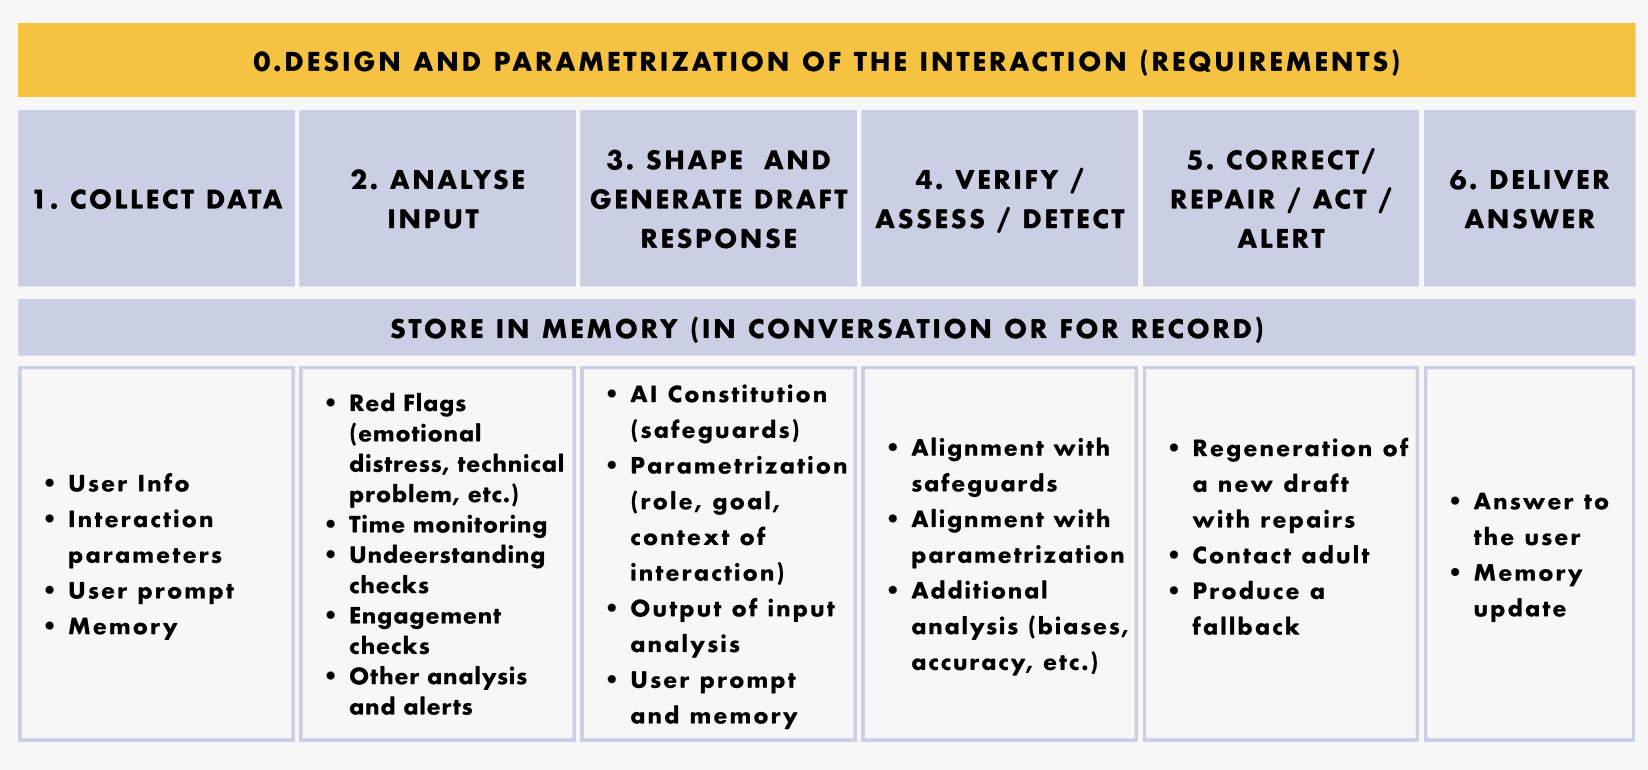
\includegraphics[width=\linewidth]{Images for manuscript/Figure 1}
\caption{Overview of the SCAFFOLD method for each turn}
\label{fig:overview}
\end{figure}

\subsection*{2.1  Designing an AI-Student interaction}

A human to human interaction is grounded in context, past experiences, time and location, guiding social norms and the behavior of the interlocutors. In interactions with AI the context is defined by the users' prompts which may or may not include additional context such as memory from past conversations or documents. In educational settings, the goal is learning and supporting development, often both in cognitive, sensory-motor and socio-emotional terms, and a successful integration of AI in educational settings needs to be able to support at least some of these learning goals.   

Lesson planning and activity design requires the educators to define the learning goals, the context, the pedagogical strategy, describing the activity and the content to cover, the flow, the structure, the rules, the assessment, etc., considering students zone of proximal development and the needed scaffolding. In a similar way, an interaction with AI, as a learning activity, needs to be defined in terms of the traditional elements of a learning activity and also in terms of the desired behavior of the LLM. For example, if a student asks for an answer to a question, should the LLM tell the answer, ask the student what he or she thinks the answer is, ask for the student's reasoning, provide a hint, or ask a metacognitive question like why are you asking this question? One can leave the decisions to the LLMs or define a scaffolding, by designing the desired interaction.     

Since it will not be possible to define all behavior in all situations, the goal is to set the key elements of an interaction with the AI in a specific learning activity and improve at each iteration. For example, a brainstorming activity of 15 year olds in the context of creating writing would rather start with the LLM asking questions about student's ideas, instead of priming for ideas generated for them. Another example is the use of an LLM to simply monitor the participation of the students in a socratic seminar, suggesting to solicit opinions of students that hadn't had the chance to express themselves. Homework support, work organization, language development, assessment support, and so many other possibilities all require a definition of specific elements of behavior. AI-student interaction design can become an opportunity to critically reflect about the pedagogical practices and students' learning.   

The list of types and examples of interaction parameters presented in figure 2 is not exhaustive and will evolve with time. The first type defines the context of the interaction, such as its setting, location, goals, interlocutors and description, allowing to integrate cultural and linguistic specificities. The second group of parameters defines the behavior of the LLM, such as desired output, pedagogical strategy, level of engagement, etc. A third group defines what happens in the background, such as what data is collected and how, what analysis needs to happen, etc. Finally, comes the learning material to consider and any other considerations not included previously. 

\begin{figure}[H]
\centering
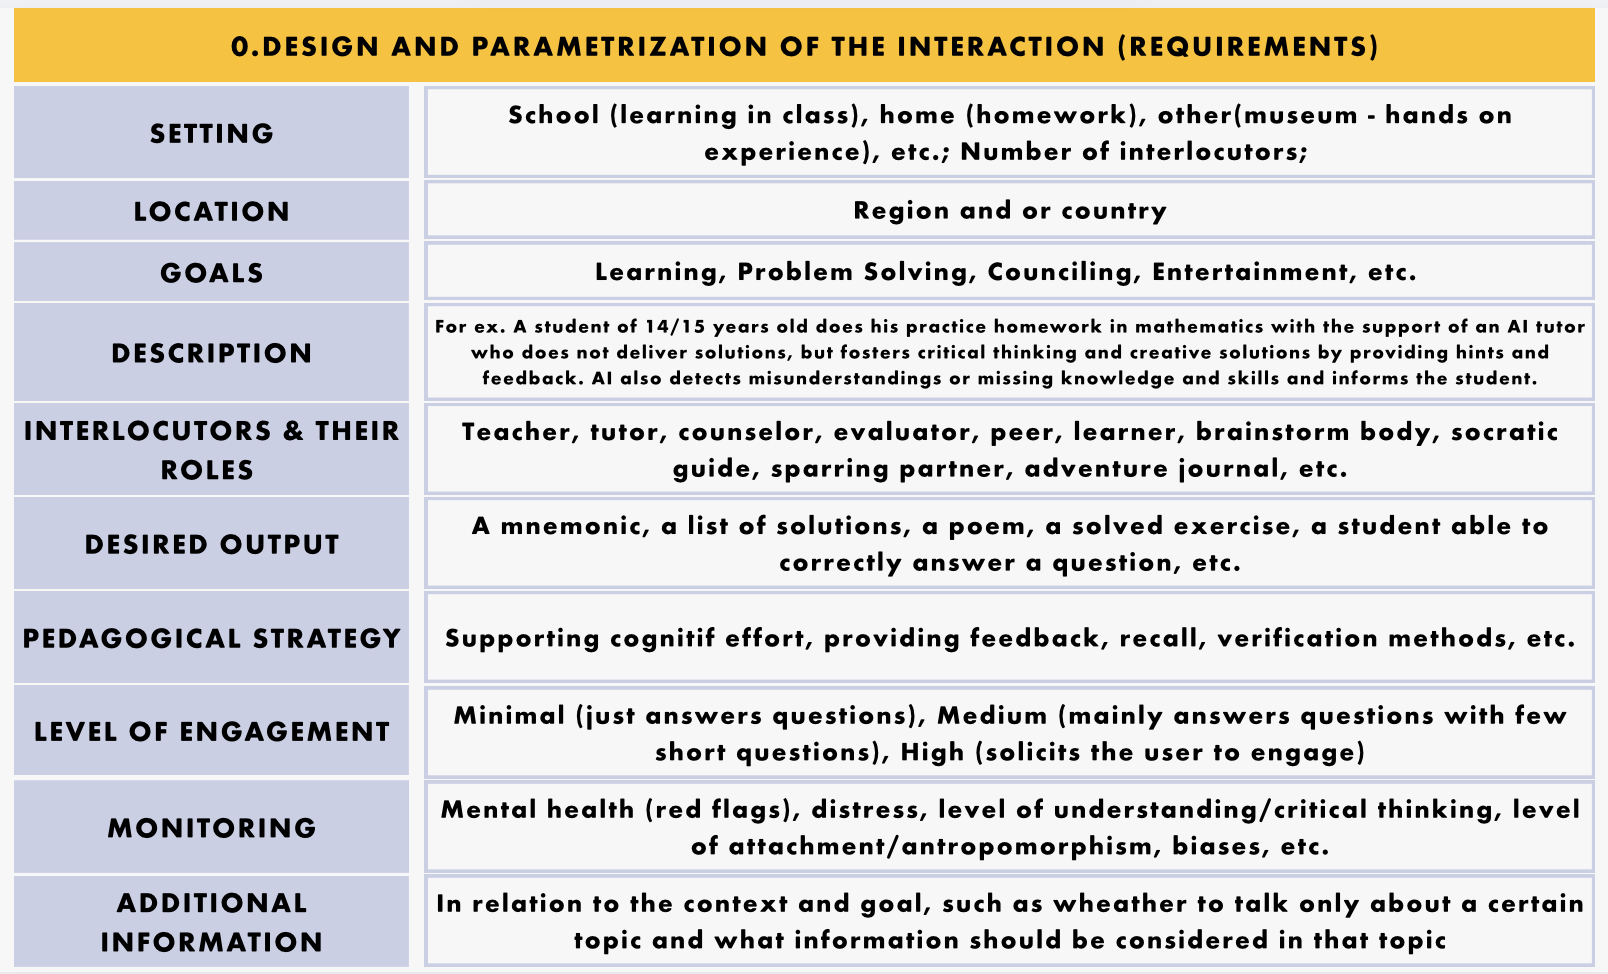
\includegraphics[width=\linewidth]{Images for manuscript/Figure 2}
\caption{Elements of a parametrization of an interaction}
\label{fig:parametrization}
\end{figure}

The interaction could be defined in a wide way and be suitable in many situations or it could be very specific to a certain use-case. Most of these parameters could be defined either as a freely formatted prompt or the users could be guided through a set of choices. The exception is the monitoring and assessment that requires more background definition and testing to be considered accurate, which, once developed, could be added to the toolbox in a modular way. 

\subsection*{2.2 Steering LLM behavior at each turn}

An LLM behaviour depends on its training datasets, size and structure of the model, its reinforcement learning from human feedback (RLHF), eventually some fine-tuning using labelled data, and the input of the model. Here we are working with existing LLMs and therefore can only act at the model's input level. However, we extend the concept of input to the model to consider several strategies such as prompt engineering and constitutional prompting (Bai et al., 2022), that is adding instructions to the user's prompt to introduce safeguards or steer reasoning as in chain of thought technique (ref); post-hoc filters (Rebedea et al., 2023), which are answer validation checks;  self-refinement methods that ask the model to critique and revise its own outputs (Shinn et al., 2023; Gou et al., 2024); external verification, that is using tools such as calculators or code compilers to run checks (Madaan et al., 2023, Pan et al., 2023, Qiu et al., 2024).  Our novel contribution is to integrate these methods in a processing flow that allows, at each turn, to analyse user's input, shape the prompt, integrate checks, produce repair or direct actions such as fallbacks or alerts, in order to achieve an acceptable level of safety for use in an educational setting.  

Specifically, SCAFFOLD framework aims at increasing LLM's reliability, addressing the intrinsic by-product of the generative nature of LLMs (Xu et al., 2025), that is the hallucinations and reduced compliance to guidelines with increasing turns as instructions get diluted (Huang et al., 2025). It is particularly important, not just to provide safe AI-student interaction and interaction that lead to learning, but also that AI provides accurate information and that teachers and students trust the system enough to consider it usable, acceptable and useful (Tricot et al., 2003).   

\begin{figure}[H]
\centering
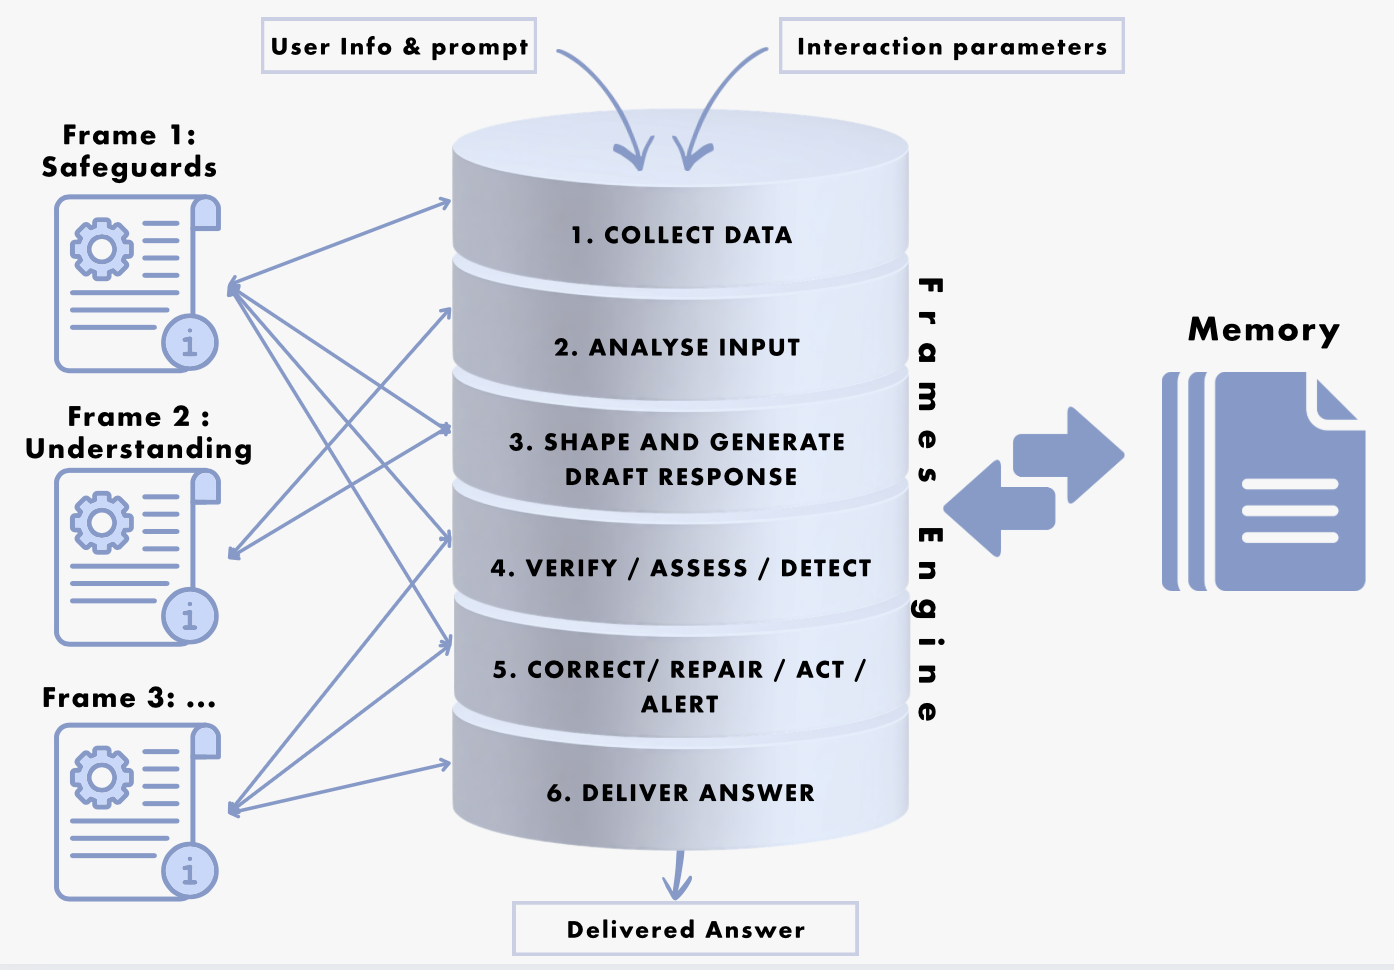
\includegraphics[width=0.7\linewidth]{Images for manuscript/Figure 3}
\caption{Illustration of the SCAFFOLD structure}
\label{fig:scaffold}
\end{figure}

The SCAFFOLD framework proposes a modular system of frames. We call a frame a coded layer between the user and the LLM that handles a set of tasks, such as a system of checks at different stages of the process, defined in the interaction. A frame could work with different LLMs and in different contexts and it communicates with a memory  The frames are compiled in a frame engine, the core of the system, which follows several steps:   
\textbf{[1: Collect data]} assembles the information from the user, such as age, nickname, location, prompt; from the designer of the interaction, such as what checks to run, what is the goal of the interaction, etc.; from memory, such as the conversation logs, previous checks results, etc. This first step feeds the others.   
\textbf{[2: Analyse input]} is a crucial and game-changing aspect of the framework. It allows to assess different levels of risks and trigger safety measures that are difficult to put in place otherwise: for example, sending an alert to a teacher when a student insists at misusing the tool or when a student is expressing dark thoughts, but also to trigger meta-responses when the user goes off topic. Another advantage of an input analysis is to be able to assess user cognitive and emotional engagement, an aspect that is particularly relevant in educational settings. Moreover, input analysis allows to perform analysis that can be used to improve the interaction in real time or to analyse the interaction afterwards. Examples of analysis can be the user's understanding of the content, progress towards a goal, level of critical thinking, level of engagement or fatigue. Some analysis can be quite simple and straightforward, such as the level of distraction from the topic, while others analysis could be much more complex and require expert validation such as in the case of detecting learning difficulties or mental health problems. In this last case, a committee of experts should contribute to the development of the analysis.    
\textbf{[3. Shape and generate draft response]} consists in shaping the prompt in a way to take into account (1) a constitution which integrates safeguards as prompts, (2) the context of the interaction – parametrisation –  with information from parametrization of the interaction and user information, (3) the results of the input analysis, and also (4) user's prompt and information from memory such as conversation logs. This step also includes the generation of a drafted response by an LLM. When the model is used in real time interaction, AI speed might become a crucial factor in deciding which model to use, while for offline analysis or when the interaction is only monitored, a more heavy model might be more appropriate.  
\textbf{[4. Verify / assess / detect]} runs validation checks on the generated draft, such as those to verify alignment with safeguards and with parametrization of the interaction. Additional analysis could be added for specific checks such as for biases, cultural pertinence, or accuracy.   
\textbf{[5. Correct/ repair / act / alert]}  considers the results of the checks in step 4 to decide the subsequent actions. For example, if the safeguards checks are not passed, it can trigger  a correct–reverify loop, a repair procedure, and regenerate an answer adding more specific instructions to the prompt and rechecking that answer until it either passes the checks or reaches a maximum number of repairs and a fallback or a notification to a responsible adult is triggered. Ideally the correct-verify loop will be what is called a non-regression safeguard, that is a repair should not re-introduce an error that was already fixed. If a repair regresses, or if the budget (iterations and time) is exhausted, the system should return a pre-approved safe fallback. The correct-reverify loop can be bypassed in certain cases such as if there is a technical problem or a red flag and in this case it would be possible to use a shortcut to a fallout asking the student to contact an adult or generating an alert or triggering reports, alerts or other actions that would notify a person of reference, and also inform the user of the action.   
\textbf{[6. Deliver Answer]}  states the final answer to deliver to the user in that turn and saves it to the memory.   
It is useful to distinguish the 2 types of checks that are used in the framework:  \textbf{deterministic checks} enforce rules that can be written in code, such as interaction time monitoring, or user's turn counting; and \textbf{probabilistic checks} use queries to a lighter or a specialized LLM, called LLM‑as‑a‑judge or AI judges (Baysan et al., 2025), (Gu et al., 2026) that can evaluate semantic and pedagogical properties, for example whether the question is on topic. These AI judges will need appropriate validations and reliability checks before deployment. Potentially a multi-agent evaluation method could be used to increase reliability and consistency, though it might be insufficiently quick for real-time conversations.     
SCAFFOLD framework needs to have an \textbf{external memory} to run effectively. The memory is needed at conversation level and can be re-initiated at each new interaction, leaving no traces. It is also possible to have a memory that tracks multiple conversations which can be useful in assessment, evaluation or personalization of the content, monitoring long term progress of students, tracking the content covered, etc. It is important to note that monitoring can be negatively perceived by the students if it is imposed and/or they are not aware of it. Monitoring can increase learning notably through teachers' changing their time allocation towards students that are more in need (Holstein et al., 2018). Monitoring can be beneficial for fostering pro-social behavior, but it can also increase anxiety (Cañigueral \& Hamilton, 2019). It is crucial to limit monitoring to when there are clear benefits for educators and students. An implementation of the framework should therefore aim at transparent practices about what is being monitored, how and who has access to that information. Users should be able to activate or deactivate memory preservation after the interaction. 

\section*{3. Pilot study: Application of SCAFFOLD in a school setting}

To explore and validate the practical deployability of SCAFFOLD, we designed a minimal SCAFFOLD framework which we piloted in two classes with children between 12 to 16 years. XXX Providing data for assessing educational value of technology. What data are we assessing? Our main goal was to explore the feasibility and usefulness of deploying SCAFFOLD in an educational setting. We additionally preregistered the following research questions:

\begin{itemize}
\item RQ1: To what extent can SCAFFOLD support children's short-term and long-term learning?
\item RQ2: How accurately can SCAFFOLD assess children's understanding?
\item RQ3: To what extent can SCAFFOLD balance students' contributions in a group?
\item RQ4: Is children's co-creation with SCAFFOLD predicted by their prior knowledge*?
\end{itemize}

* We originally preregistered the length and depth of the created mnemonic as an indication of children's knowledge, however since a posteriori length and depth were not representative of children's engagement because the mnemonics were sometime created by the LLM, we decided to use another indicator that we defined priori to the registration –  the level of co-creation with the LLM – which reflected better children's involvement and participation.

\subsection*{3.1 Methods and materials}

\subsubsection*{3.1.1 Participants}

We recruited two classes from a rural German comprehensive school, consisting of 27 children (M = 13.46 years, SD = 0.81, 4 female, 21 male, 2 other/not specified) and two teachers (M = XX, SD = XX, 2 female). We lost the LLM interaction data of one group and therefore report findings for 24 students and nine groups. Participants were German native speakers and provided written (parental) consent. The experiment was approved by the local ethics committee (25 ETHICS-247).

\subsubsection*{3.1.2 Marty robot}

Marty is a medium-sized, educational humanoid robot, with movement and speech capabilities, designed to support STEAM education. Marty features a unique walking mechanism and individually powered limbs, enabling it to walk, turn, dance, sidestep, kick a ball, and perform expressive movements. Designed for learners as young as 4, Marty supports progression from screen-free programming to block-based and text-based coding (Python), making abstract coding concepts tangible through physical embodiment (\url{https://robotical.io/about/all-about-marty/}).  A custom web interface was deployed for this study, based on the standard Robotical web application (\url{https://webapp.robotical.io}). The interface was modified to integrate the SCAFFOLD pedagogical framework and support the experimental design requirements.

\subsubsection*{3.1.3 Description of Marty's SCAFFOLD design}

Marty's SCAFFOLD design was set to last 10 minutes and follow three phases: (i) First, students were prompted to select the microcontrollers concepts to include in the mnemonic; (ii) in the second phase, students co-create the mnemonic with Marty; and (iii) in the third phase students should memorize the mnemonic. The parametrization of the interaction is described in \textbf{Figure 5}. Because the initially set time was too little, groups did not reach the third phase.

We developed the general architecture to run the 6 SCAFFOLD stages (collect data, analyse input, shape and generate draft response, verify, repair and deliver answer) that are described in supplementary material S1. While this architecture can run on any LLM model, we used gpt-4.1-mini on Microsoft Azure for this pilot. Since the interaction involved the social robot Marty, we additionally deployed text to speech and speech to text by using a Microsoft Azure male standard voice.

\begin{figure}[H]
\centering
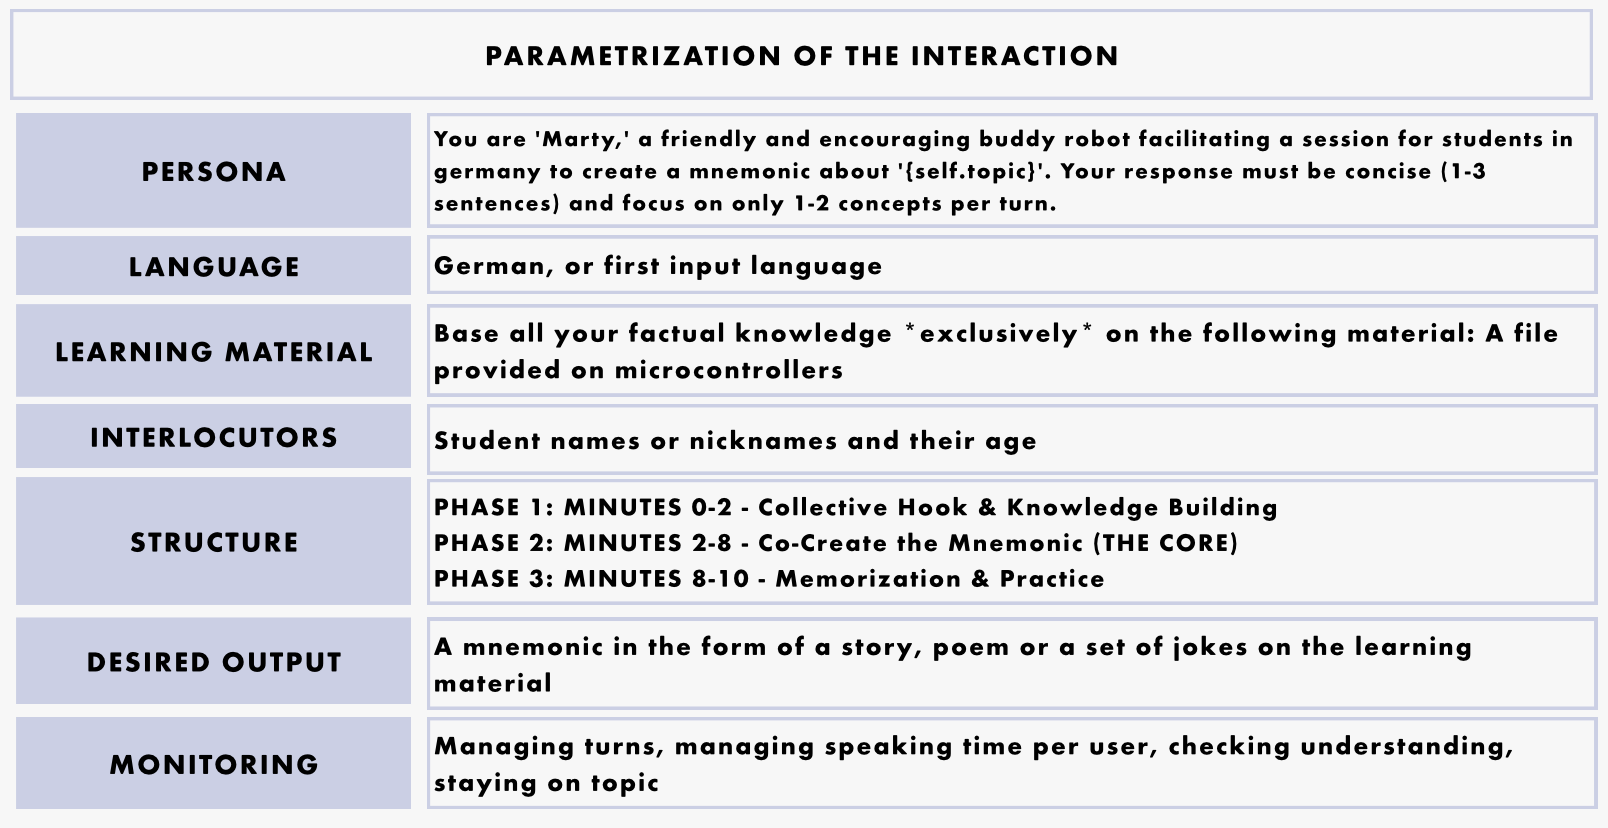
\includegraphics[width=\linewidth]{Images for manuscript/Figure 5}
\caption{Marty's interaction parameters}
\label{fig:marty-params}
\end{figure}

We created five frames detailed in table 1: the main frame  "Mnemonic CoCreator Frame" (1),  which managed most of the checks, and four more specific validation frames. The "language checker" frame (2) assessed  age appropriate language, tone, and complexity of responses. The "balanced turns" frame (3) managed fair turn-taking across students, tracking participation count, speaking time, and consecutive turns. The "comprehension tracker" frame (4) maintained per-student, per-concept understanding profiles, tracking whether each student understands, is confused about, or has misconceptions regarding specific concepts. Lastly, the "phase checker" frame (5) ensured that responses align with the current session phase goals and pedagogical requirements (see supplementary material S2 for more details).

\begin{table}[H]
\centering
\begin{tabular}{|l|p{5cm}|p{5cm}|}
\hline
\textbf{Frame} & \textbf{Responsibility} & \textbf{Key Checks} \\
\hline
Mnemonic CoCreator & Session management, phase transitions, mnemonic building & Time-based phases, contribution analysis, mnemonic quality \\
\hline
Language Checker & Age-appropriate language & Complexity, tone, technical terms usage \\
\hline
Balanced Turns & Fair participation & Turn counts, speaking time, monopolization detection \\
\hline
Comprehension Tracker & Understanding monitoring & Per-student, per-concept profiles \\
\hline
Phase Checker & Phase alignment & Phase-specific goals and pedagogical requirements \\
\hline
\end{tabular}
\caption{\label{tbl:frames}Overview of frames with their responsibility and key checks}
\end{table}

The frames communicated via a \texttt{shared\_context} dictionary for ephemeral data within a turn and a \texttt{frame\_memory} dictionary for persistent state across turns. Prior to the pilot deployment, the framework was tested in 3 ways: manually, with static simulations, and with dynamic simulations using three student personas impersonated by another LLM (see  supplementary material S3 for more details).

\subsubsection*{3.1.4 Procedure}

The pilot was conducted as part of an experimental study (Leisten et al, in prep.), in which students participated in a 7-weeks AI literacy training centered around building and interacting with the social robot Marty (\href{http://Robotical.io}{Robotical.io}). The curriculum covered topics such as artificial intelligence (AI), Large Language Models (LLMs), social robots, programming, sensors, and microcontrollers. We deployed the SCAFFOLD framework in the last session of the 7-weeks curriculum. Students worked in randomly assigned groups of 3-4 to create a mnemonic (a poem, a story or a few jokes) about microcontrollers with the support of Marty. A summary of the microcontrollers learning materials covered in class was provided both to students and the LLM. First, students created a mnemonic using the LLM out of the box. Students then created a second mnemonic with the SCAFFOLD framework enabled. Each mnemonic session lasted approximately 10-15 minutes.  
We administered pre-, post-, and feedback surveys in Qualtrics (Qualtrics, 2024) to students at several timepoints during the 7-weeks curriculum. Here, we report the results relevant for the evaluation of SCAFFOLD, specifically, children's knowledge about microcontrollers, assessed in the pre-test (conducted at week 1; T1), post-test (conducted at week 7; T2), and the learning retention test (conducted 7 weeks after T2; T3), as well as students' and teachers' feedback about the LLM interactions. All code and data are available on \href{https://github.com/OlgaMuss/LLM_Frames_Paper\%20}{github} and a simulation app on \href{https://buildbot-4tzkvoxzssupnzkb9e6va4.streamlit.app}{streamlit cloud}. More detail on the methodology can be found in the Supplementary Materials S4.

\begin{figure}[H]
\centering
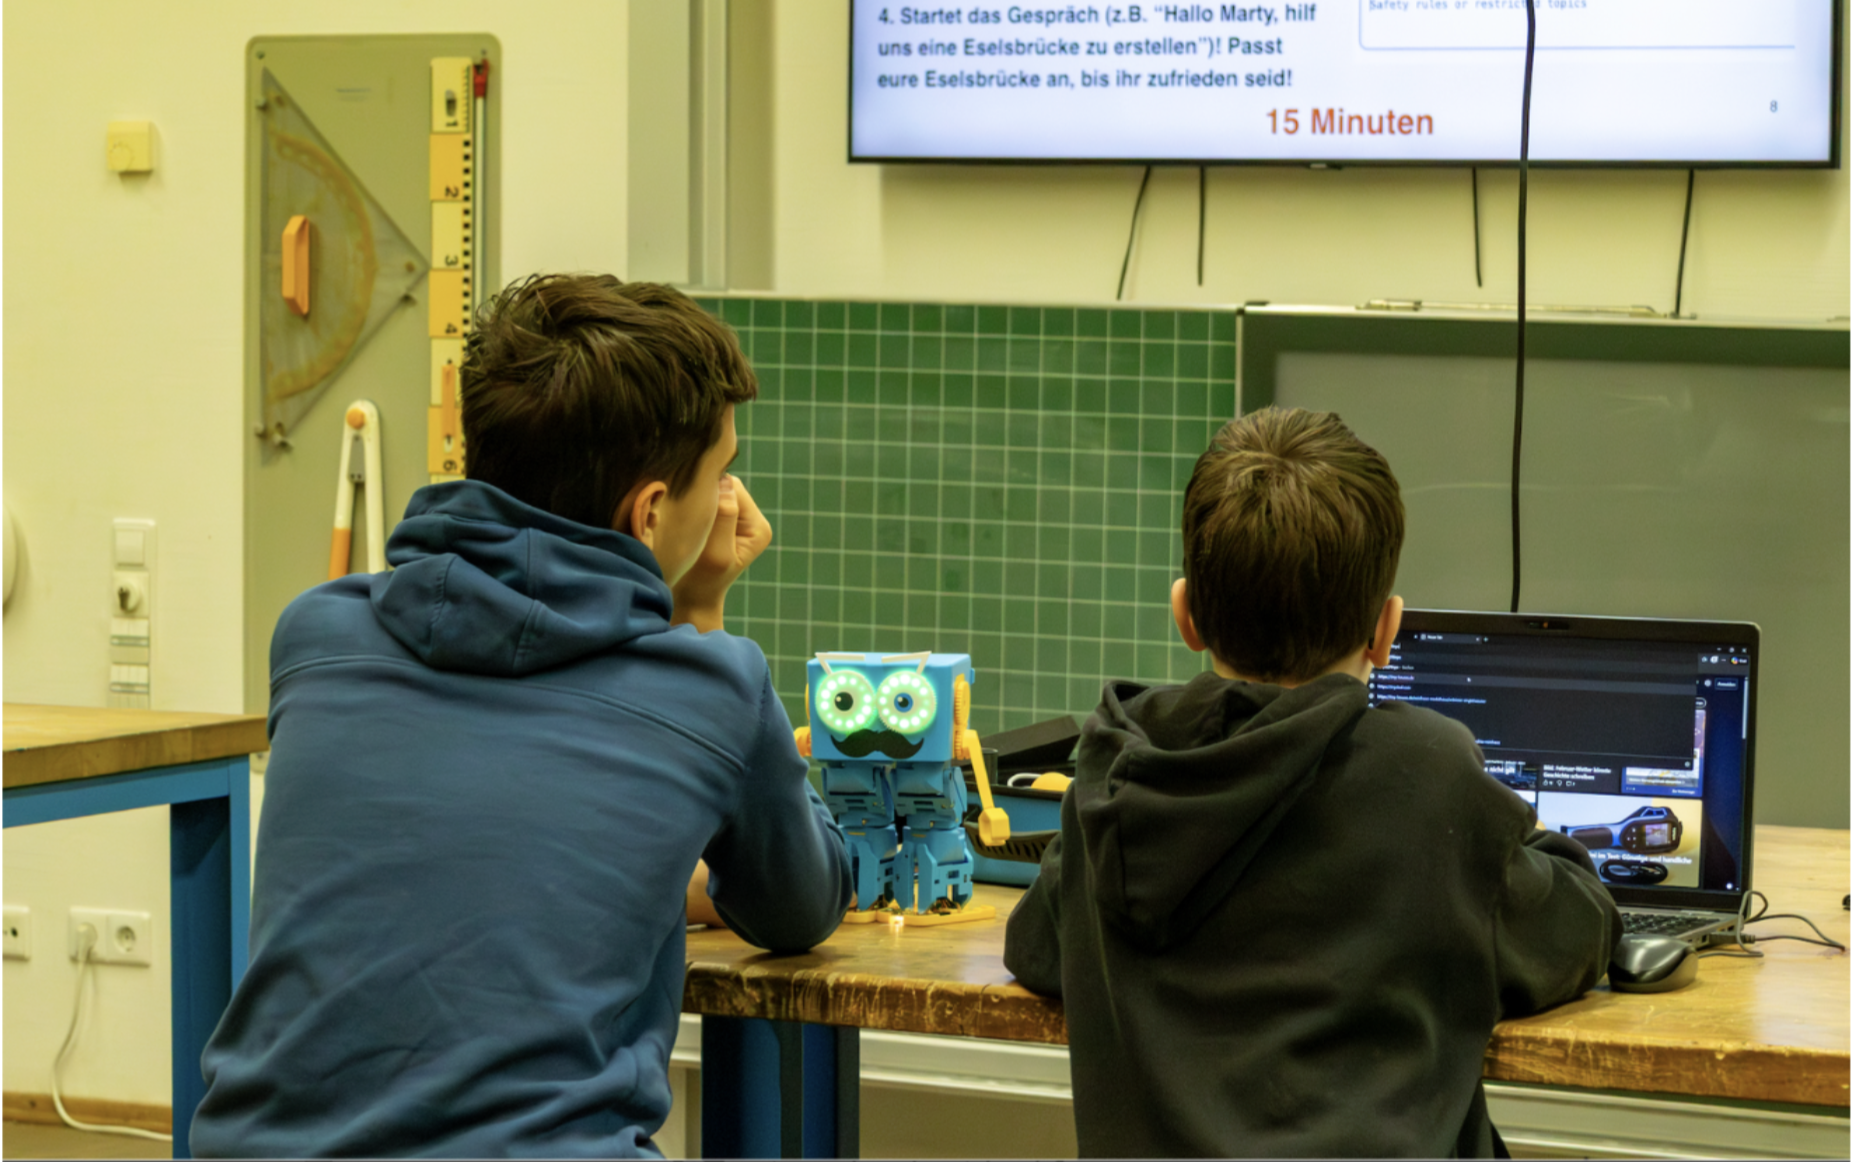
\includegraphics[width=0.8\linewidth]{Images for manuscript/Figure 4}
\caption{Illustration of the setting of the interaction}
\label{fig:setting}
\end{figure}

\subsubsection*{3.1.5 Measurements}

\textbf{Students' microcontroller knowledge.} We assessed students' microcontroller knowledge at T1 with two questions and added another eight questions at T2 and T3, based on the learning materials covered in class (see Supplementary Materials S4 for items). The single-choice questions covered what a microcontroller is, its function, components, and a few technical details (voltage, pins, programming language). Children were instructed to select one out of five answer options (one of them being "\textit{I don't know}") for each item, resulting in a possible score of 0-2 at T1, and 0-10 at T2/T3 (1 = correct, 0 = wrong, 99 = don't know, later coded as 0 for main analyses).

\textbf{Students' perception.} We assessed students' intrinsic motivation after the session using a shortened and adapted version of the intrinsic motivation inventory (Deci \& Ryan, 1985, Wilde et al., 2009), previously used by Heindl (2020) and Röllke \& Großmann (2022) in children's samples. In eight items, students' indicated their perceived enjoyment, competence, tension, and usefulness of the class activities on a 5-point Likert scale (1 = does not apply, 5 = applies fully). Additionally, we added five questions specific to the LLM interaction, in which we asked about enjoyment, perceived learning gains, and equal contribution of team members on a 5-point Likert scale (1 = very bad / very little / not at all, 5 = very good / very much / absolutely), and two open-ended questions for positive and negative feedback.

\textbf{Teachers' perception.} Teachers completed a feedback survey after the session, including 12 quantitative questions assessing perceived student engagement and learning, difficulty, and items specific to the LLM interaction (e.g., helpfulness, difficulty, entertaining). Additionally, teachers provided open-ended positive and negative feedback.

\textbf{LLM interaction measures.} We collected Marty's interaction logs to analyse students' interactions with the LLM. These logs included session IDs, timestamps, LLM instructions, user and system prompts, turns, and students nicknames. The SCAFFOLD logs additionally included the frames meta data as described below. The students' interaction logs with their social robot were analysed manually, describing each turn and noting students' when students proposed ideas or concepts relevant to the mnemonic. 

\textit{Contributions and off-topic turns}   
Each student prompt was manually assessed noting if what students said was on or off topic to the task, if it was a concept to include in the mnemonic and which concept, if it was a constructive idea for the creation of the mnemonic. Contributions are students' proposed concepts or relevant ideas. Off-topic turns are students' prompts that are unrelated to the task on hand.   

\textit{Balanced turns}  
For each conversation, we noted the number of turns each student spoke, and then used the Gini coefficient to estimate equity of turns with the following formula: G = $\Sigma$(2i-n-1)*x\_i / (2*$\Sigma$x\_i*(n-1)) (Dixon et al., 1987).

\textit{Co-creation level}  
While we pre-registered the length and depth of the created mnemonic as an indicator of learning success, we later realized that the mnemonic was sometimes created by the LLM and therefore did not represent students' engagement or contribution. We therefore decided to use another variable that we defined at the pre-registration: the co-creation level ( "0: LLM did it all, 1: concepts by kids/rest LLM, 2: concepts by the students, co-creation of the mnemonic, 3: mainly by students). This variable was coded manually counting students' contributions to each phase and considering the depth of contribution (e.g. one very simple concept vs several complex ones). We added a 0.5 level a posteriori to integrate the case where students contributed in guiding the LLM, but not on the concepts related to the topic of learning. 

\subsubsection*{3.1.6 Data analysis}

Statistical analyses were performed in R (R Core Team, 2020) using RStudio (Posit team, 2025) and Python 3.12.12 (Python Software Foundation, 2021) using Jupyter Notebooks (Kluyver et al., 2016). Since the aim of this pilot was to test the feasibility and potential benefits of SCAFFOLD, statistical analyses are mainly descriptive. To answer RQ1 and RQ4, we fit a linear mixed-effects model with children's post-test knowledge scores (T2: immediate post-test; T3: delayed post-test) as the outcome, co-creation level and timepoint (immediate vs. delayed) as fixed effects, and participant as a random effects to account for repeated measures and controlled for prior knowledge (T1). We fit a linear mixed-effects model using the lmer() function from the lme4 package (Bates et al., 2015) with p-values computed using the lmerTest package (Kuznetsova et al., 2017). We originally preregistered separate linear mixed effects models per timepoint, which we ran and their results are available in supplementary material S5. However a combined model allows to account for repeated measures, to increase statistical power and to control for prior knowledge and therefore has been chosen for reporting.

\subsection*{3.2 Results}

The aim of this pilot was to test the feasibility, usability, and utility of the frame for supporting children's learning. We were able to implement the framework, enabling students to co-create a mnemonic with a social robot, highlighting the feasibility and usability. Below, we report the findings organized by relevance, including both descriptive findings and preregistered analyses.  

\begin{figure}[H]
\centering
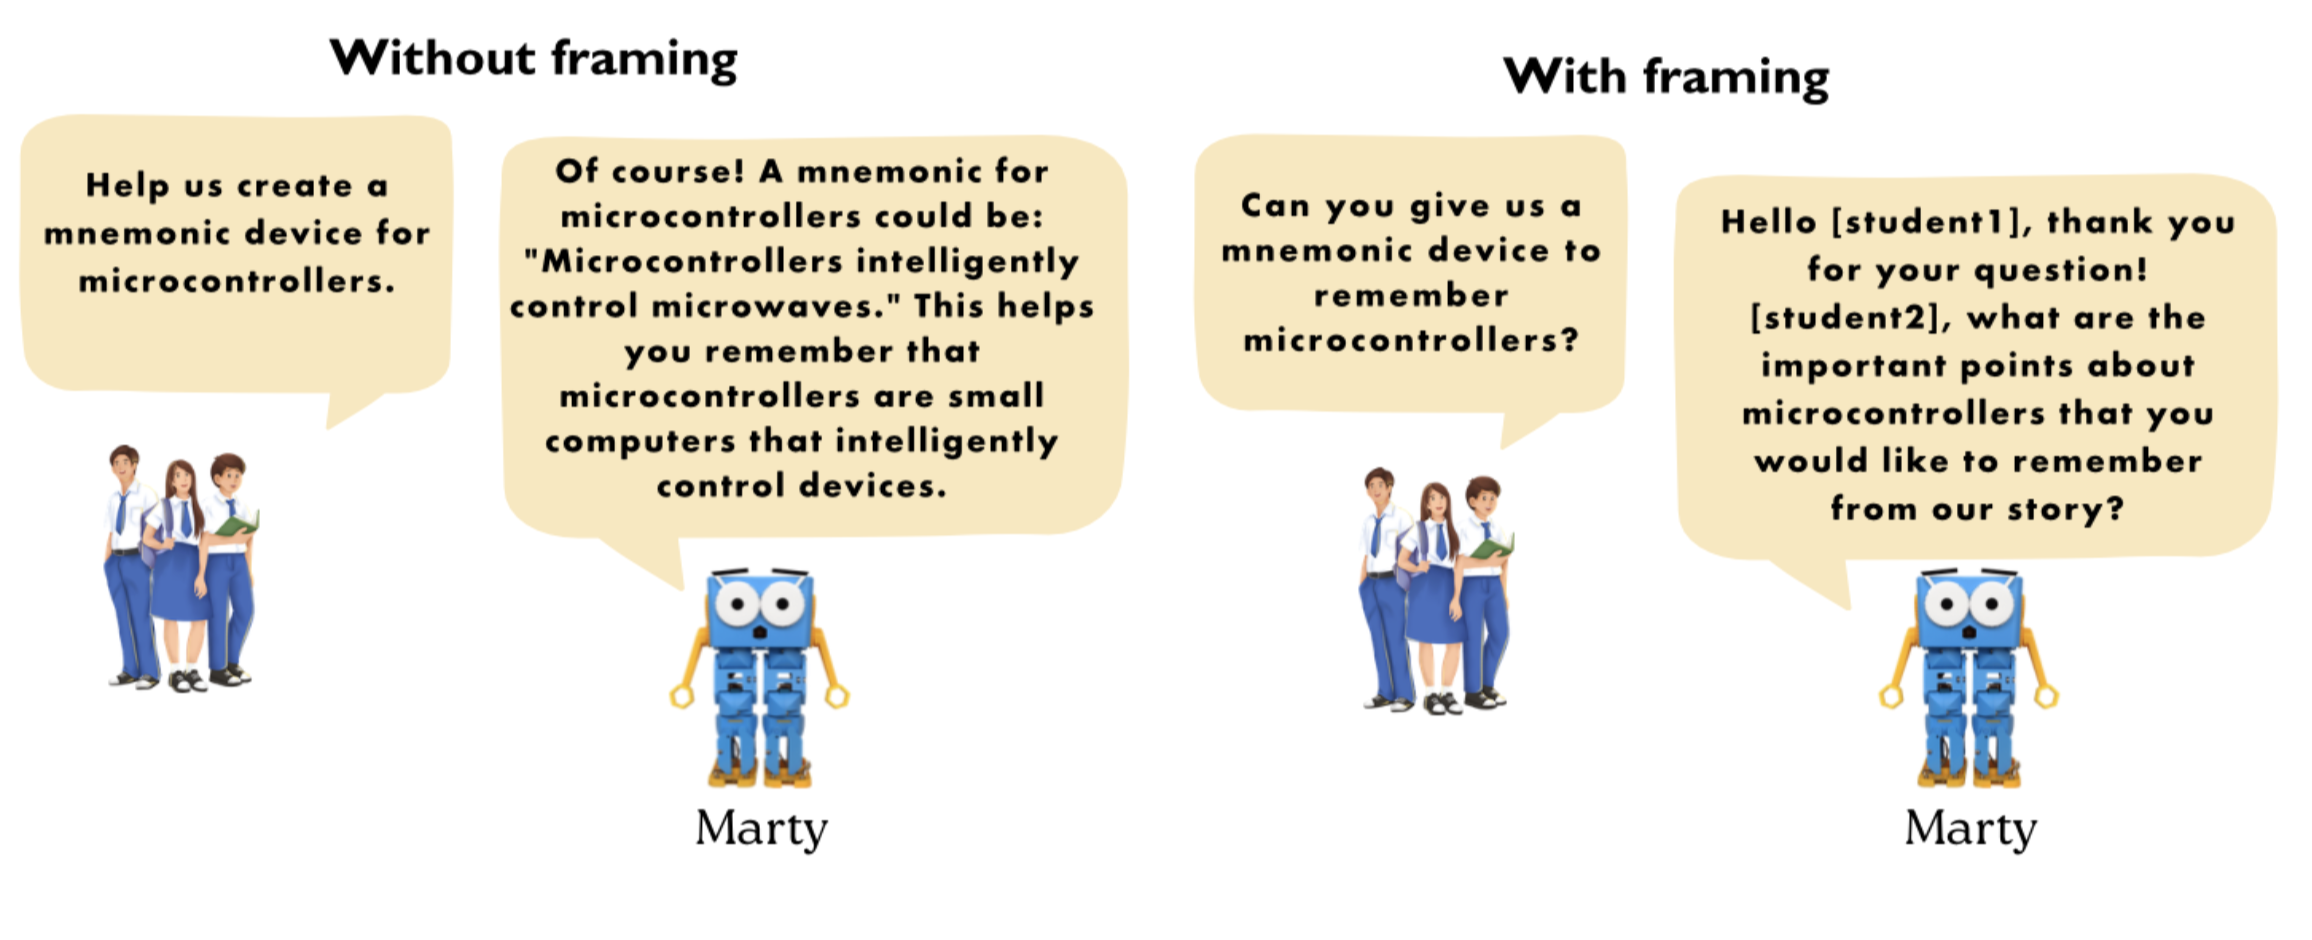
\includegraphics[width=\linewidth]{Images for manuscript/Figure 6}
\caption{Example of answers without and with SCAFFOLD framing}
\label{fig:comparison}
\end{figure}

\subsubsection*{Finding 1 : Students were more active with SCAFFOLD than without}

The main impact of the SCAFFOLD frame was that students contributed to the creation of the mnemonic, a behavior that was absent from their LLM interactions without the framing. Students contributed to the identification of concepts to include in the mnemonic (18 relevant suggestions by 13 out of 24 students) and to the actual creation of the mnemonic (13 suggestions from 12 out of 24 students, \textbf{Figure 7}). This is an important shift from students being mere consumers of AI technology to becoming active creators.

\begin{figure}[H]
\centering
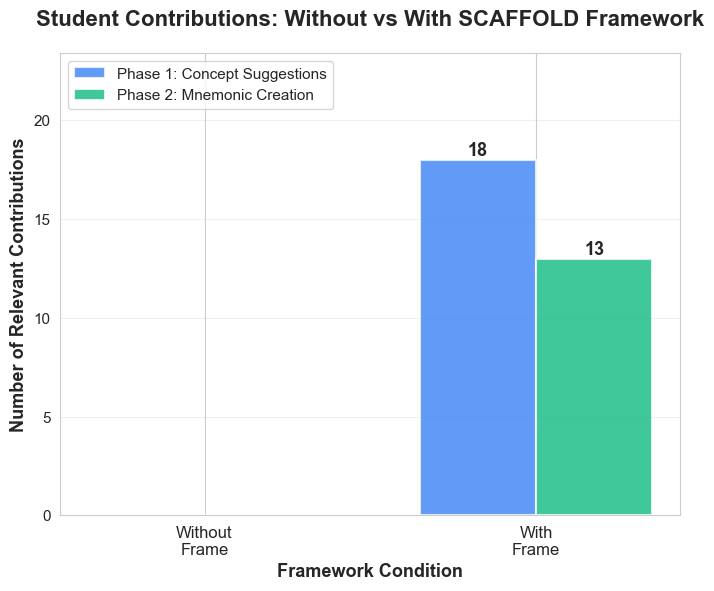
\includegraphics[width=0.7\linewidth]{Images for manuscript/Figure 7 contributions}
\caption{Students' contributions per phase with and without the SCAFFOLD framework}
\label{fig:contributions}
\end{figure}

While all groups successfully created a mnemonic, two groups fully co-created it, two groups provided the concepts with the LLM proposing a mnemonic, one group provided input for the creation of the mnemonic. The remaining four groups provided only limited input to the mnemonic creation.

\subsubsection*{Finding 2: SCAFFOLD supports more balanced turn taking (RQ3)}

Another important aspect was a more balanced involvement of students (RQ3). Without SCAFFOLD, 6 students did not participate in the interaction at all, while only one student did not participate in interaction with SCAFFOLD. While participation was not significantly more equitable (\textit{W} = 9.00, \textit{p} = .13), the balance between turns was more reliable (i.e., varied less; \textit{F} = 5.84, \textit{p} = .02) as indicated by the GINI Coefficient (Dixon et al., 1987), the standard equity measure in economics (see \textbf{Figure 8}). From this exploratory analysis, the balanced turns frame appears to have worked well and succeeded in guiding a more balanced interaction, setting an example for multi-user interactions with AI.  

\begin{figure}[H]
\centering
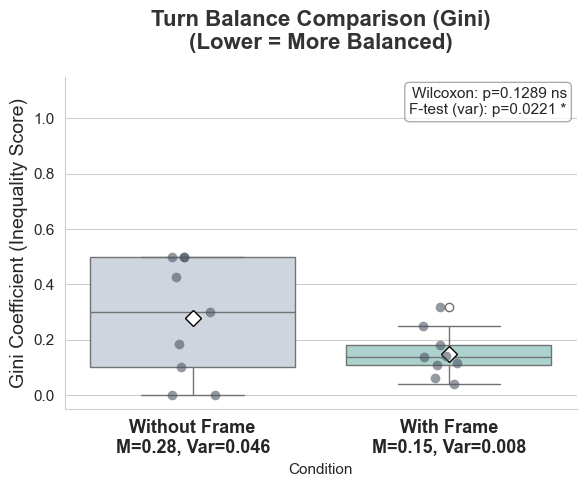
\includegraphics[width=0.65\linewidth]{Images for manuscript/Figure 8 gini}
\caption{Gini Coefficient (Dixon et al., 1987) assessing the level of equitable participation in interaction without or with SCAFFOND framing. The dots represent Gini coefficients per group.}
\label{fig:gini}
\end{figure}

\subsubsection*{Finding 3: Higher co-creation level is associated  with higher post-test knowledge scores and is not predicted by their pre-test level (RQ1 \& RQ4)}

Children's microcontroller knowledge was significantly and positively predicted by co-creation level (\textit{b} = 1.06, \textit{SE} = 0.35, \textit{p} = .005; \textbf{Figure 9}), indicating that higher student engagement during mnemonic creation was associated with better learning outcomes. This effect remained significant when controlling for prior knowledge (T1), which itself did not predict post-test scores (\textit{b} = -0.13, \textit{SE} = 0.49, \textit{p} = .79; \textbf{Figure 9}). There was no significant main effect of timepoint (\textit{b} = -0.09, \textit{SE} = 0.63, \textit{p} = .88), suggesting similar overall performance on immediate (T2) and delayed (T3) post-tests. The co-creation and timepoint interaction was not significant (\textit{b} = -0.59, \textit{SE} = 0.38, \textit{p} = .13), indicating that while the co-creation effect showed a trend toward weakening over time (from +1.06 at T2 to approximately +0.47 at T3), this difference was not statistically significant. The model accounted for substantial individual variation (participant-level variance = 1.77, residual variance = 1.94).

\begin{figure}[H]
\centering
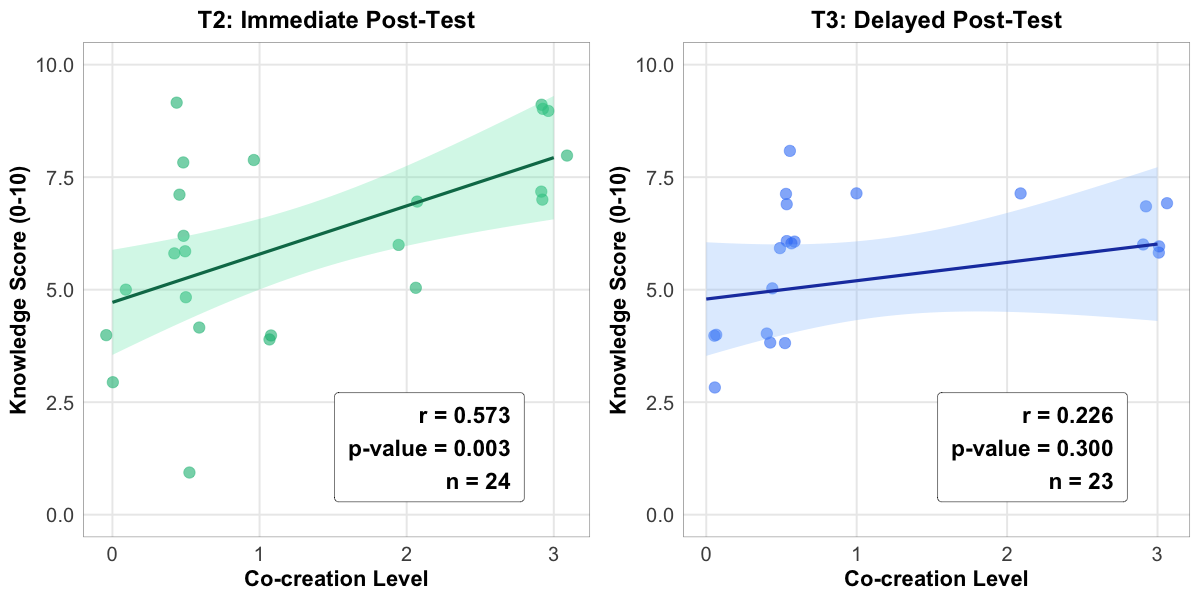
\includegraphics[width=0.8\linewidth]{Images for manuscript/Figure 9 T2 and T3}
\caption{Correlation between co-creation level with microcontrollers' knowledge score on 10 items at T2 – the same day post-test and at T3 – 7 weeks after. Co-creation level defined as:  0: LLM did it all, 0.5: some guidance from students unrelated to learning, 1: concepts by students/rest LLM, 2: concepts by the students, co-creation of the mnemonic, 3: mainly by students) and their results on Micro-controller knowledge at post test.}
\label{fig:correlation}
\end{figure}

\begin{figure}[H]
\centering
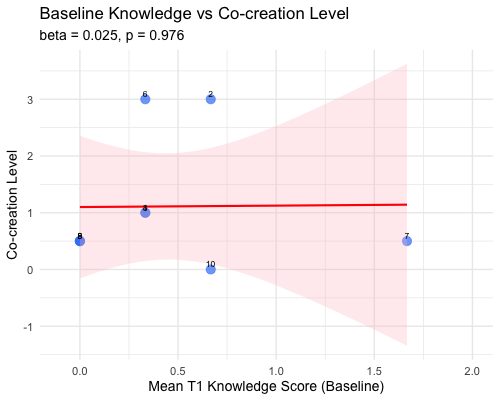
\includegraphics[width=0.6\linewidth]{Images for manuscript/Figure 11 T1}
\caption{Linear Model for Co-creation\_Level $\sim$ mean\_T1\_score per group which is the knowledge scores on 2 questions on microcontrollers at T1, the pre-test performed several weeks before the interaction. Co-creation level of the mnemonic defined as 0: LLM did it all, 0.5: some guidance from students unrelated to learning, 1: concepts by students/rest LLM, 2: concepts by the students, co-creation of the mnemonic, 3: mainly by students).}
\label{fig:prior-knowledge}
\end{figure}

\subsubsection*{Finding 4: SCAFFOLD reduces off-topic turns}

Students' off-topic turns decreased from 38\% without the framing to 1\% with SCAFFOLD (\textit{W} = 0.00, \textit{p} = .03; \textbf{Figure 11}). This suggests that students were more engaged in the activity, potentially because Marty was asking individual students directly. The reasons behind this increased on-topic contributions would need to be further investigated. 

\begin{figure}[H]
\centering
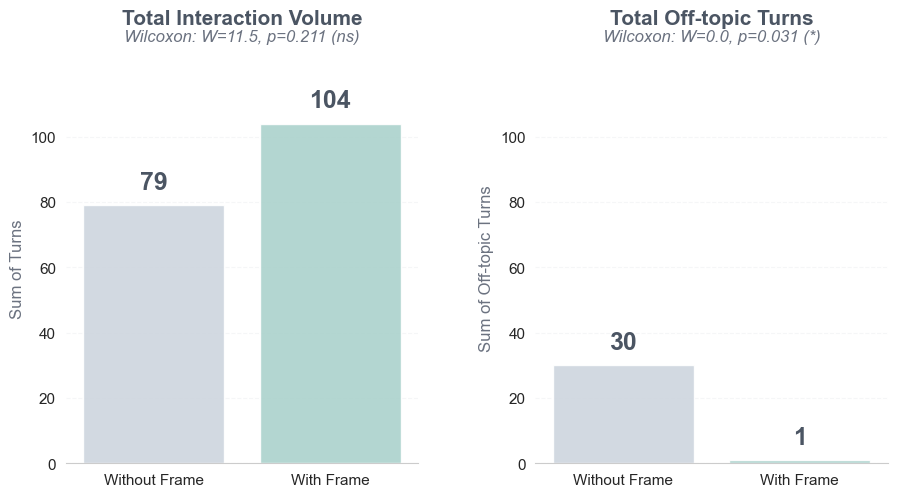
\includegraphics[width=0.6\linewidth]{Images for manuscript/Figure 10 off topic}
\caption{Total number of turns in general and turns off-topic without and with SCAFFOLD framing}
\label{fig:offtopic}
\end{figure}

\subsubsection*{Finding 5: Students and teachers enjoyed the activity}

In general students rather enjoyed the activity (\textit{M} = 3.96/5, \textit{SD} = 0.92) and thought that the LLM interaction has helped them learn (\textit{M} = 3.27/5, \textit{SD} = 1.12, \textbf{Figure 12}), with several students reporting creation as a mnemonic with Marty as what they liked about the LLM interaction with SCAFFOLD. Negative feedback came mainly from groups that ran out of time, which resulted in Marty resisting to answer and instead indicating that their time was over. Both teachers also considered the activity helpful (score 3 out of 4 for both) and somewhat engaging (score 4 out of 5 for both).

\begin{figure}[H]
\centering
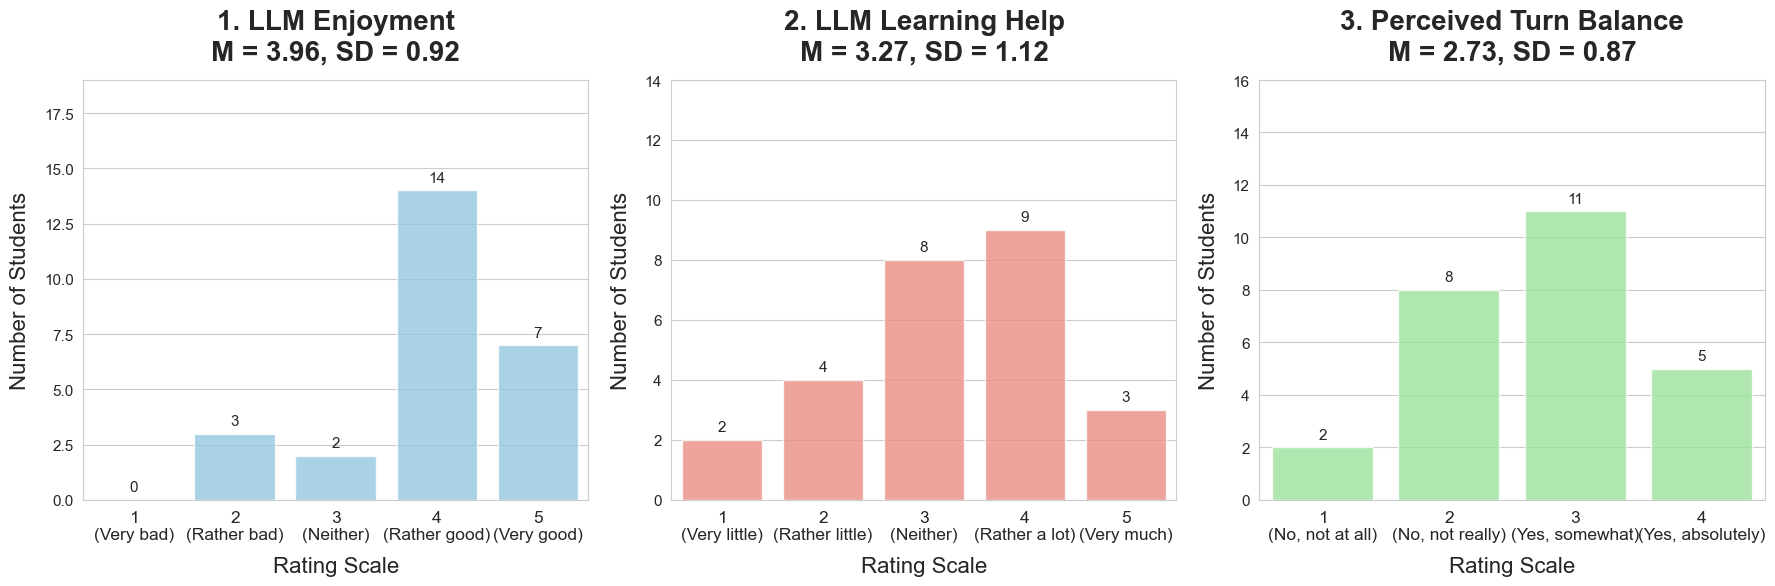
\includegraphics[width=\linewidth]{Images for manuscript/Figure 12}
\caption{Students feedback on the interaction with Marty using SCAFFOLD: 1. LLM enjoyment: How did you like your last voice interaction with Marty? (1-5), 2. LLM Learning Help: How much did your last conversation with Marty help you learn? (1-5), 3. Perceived Turn Balance: Did you feel everyone talked to Marty equally? (1-4)}
\label{fig:feedback}
\end{figure}

Overall, the pilot showed potential for engagement and learning, and while the developed framework is far from perfect, it was an improvement from the standard LLM interaction without framing.

\section*{4. Discussion}

In this paper, we present a novel methodology, SCAFFOLD, that supports the implementation of safer and more beneficial LLM interactions in an educational setting. SCAFFOLD is independent of the underlying LLM, allowing the open-source community to develop an ecosystem of safeguards and model behaviors in collaboration with educators and child psychologists. Safe and helpful LLMs are essential for delivering effective AI literacy to students and teachers, and also to harvest the potential of this technology to improve well-being, learning and human relations. The methodology allows to envision an AI technology implementation in education that goes beyond students sitting at their desks in front of a screen working individually, and towards a more dynamic and social learning, supporting multi-user interactions with an AI or simply by assisting teachers in analysing conversations with or between students. The modularity and control over the data storage and processing, and therefore data privacy is another advantage allowing to minimise data sharing while delivering the benefits of personalisation and differentiation.  
We also piloted SCAFFOLD in a short multi-user interaction in a classroom setting with 12-16 year olds, showing feasibility and a potential for learning improvement and engagement. We saw that students were more engaged with the framed AI, proposing concepts and ideas, a behavior absent without the framing. With the framed LLM, students stayed on topic and, while  the reasons behind this increased on-topic contributions would need to be further investigated, it seems natural that once the LLM provided the mnemonic for the students they tended to move to a new exploration, while a framed LLM, instructed to redirect if someone goes of topic, which happened once, helped students to stay on the task.   
Students also shared reliably more equitably their turns at speaking with the LLM, notably because the LLM asked questions directed at individual students using their nicknames, even if they didn't always, but most of the time, respected the guidance. It is important to note that, ideally, an interaction would imply minimal input from an AI, with students working out the mnemonic as autonomously as possible. This would mean that several students might speak one after another, with no intervention from the LLM. While this is possible in general – we tested that in the prototype version – we were not able to implement it due to time constraints. Since this analysis did not take into account turns of the LLM itself, which are by design at each turn, further research should explore how allowing users to speak one after another with the AI intervening only when needed, could balance speaking time not only between students but also between students and AI.  
Students that contributed more to the mnemonic, those with higher co-creation level, also had higher post-test scores, suggesting that the framing of LLM could have a potential to support learning. The results hold by controlling for pre-test knowledge suggesting that the LLM interaction might support learning regardless of the initial level of the learner. While we didn't expect to see these positive results in such a short exercise, these are consistent with the retrieval practice in the literature (Roediger \& Butler, 2011): remembering strengthens retention. More future research is needed to evaluate the potential of a framed LLM to support learning.   
Our exploratory piloting and analysis have several limitations. In our setting SCAFFOLD failed to accurately assess understanding. In part, this is due to the little input from the students because of the short time they had per person, in part because we haven't defined well enough how the statistical checker should assess understanding. This topic is very complex and would benefit from further research.   
Moreover, the interaction was too short to reach the third phase when the students were supposed to practice the mnemonic. While the closure worked well at first, we didn't define what should happen if the students kept interacting with Marty. In the future, it would be useful to add a strong cutoff when the interaction stops completely. Also, some students indicated that they would have loved to explore other topics with Marty, which is a legitimate wish and we probably should have added an exploration session before jumping into a structured interaction.  
Finally our study is characterized by a small, homogenous sample, limited interaction time with the LLM, and a limited impact assessment. The piloted frame is a first step towards a usable version that should be tested and improved iteratively with the involvement of educators and experts. For example, the balanced turns frame was reliably successful in its task to ensure balanced turns between students, while the comprehension checker frame needs further development to include multi-dimentionality of learning and empirical validation of the accuracy of the statistical checks. We cannot generalize from our data, but simply point to a potential for further research, a research that is crucial when the largest proportion of those using LLMs are teenagers without proper training and safeguards from the service providers or regulators in most cases.

\section*{Acknowledgements}

Teachers, students, robotical.ai team 

\section*{Competing interests}

Authors did not receive funding for this work.

\bibliography{references}

\section*{Annexes}

\subsection*{Supplementary materials: \url{https://github.com/OlgaMuss/LLM_Frames_Paper}}

\begin{itemize}
\item S1: Framework Architecture
\item S2: Frame implementation
\item S3: Testing
\item S4: Classroom pilot methods
\item S5: Pilot statistical analysis
\item S6: Learning material
\item S7: Codebook for qualtrics
\item S8: \href{https://docs.google.com/document/d/1H8ze6IJ8H7I5qsTjTcrK8b4FXwIk0rf9yr8sr4EKXkY/edit?tab=t.0}{Detailed Buildbot LLM Interaction analysis}
\item S9: \href{https://github.com/OlgaMuss/LLM_Frames_Paper/blob/main/Data_analysis/Data/BuildbotAnalysis\%20-\%20LLM\%20analysis.csv}{LLM interaction coding and co-creation level calculation}
\end{itemize}


\subsection*{Other links:}

\begin{itemize}
\item \href{https://github.com/OlgaMuss/LLM_Frames_Paper\%20}{github}
\item simulation app on \href{https://buildbot-4tzkvoxzssupnzkb9e6va4.streamlit.app}{streamlit cloud}
\item pre-registeration: 10.17605/\href{http://OSF.IO/K7UE2}{OSF.IO/K7UE2}
\end{itemize}

\subsection*{Statement on GenAI use}

\begin{itemize}
\item This paper has been written without the help of an AI. After writing, Gemini was used for proofreading.
\item We used Cursor with several models for fine-tuning and debugging the frame's code.
\item We used Claude for a first draft of the supplementary materials S1, S2 and S3 generation based on the existing code, which we reviewed and adjusted afterwards.
\item We used Cursor to assist in writing data analysis code which we checked carefully and modified as needed.
\end{itemize}

\subsection*{Authors contributions}

\textit{Olga Muss} (Education and cognitive sciences: specification of inputs and steps'' tasks, designing the interaction for the interaction, testing the frame prototype and the final frame, writing of the paper)

\textit{Luca Leisten} (HCI and learning expertise: Designing and implementing the educational intervention at the school, reviewing the frame design, prototype and implementation, writing of the paper)

\textit{Charles Edouard Bardyn} (Technical expertise: idea of the SCAFFOLD Framework, development, patent, specifications, creation of a prototype, coding of the framing, writing of the paper)

\end{document}
